\documentclass[main]{subfiles}

\begin{document}
      \subsection{Вычисление главных направлений.}
    M --- поверхность, $X_0$ --- точка M, в $X_0$ опр
    \[E,F,G \text{ - \RNumb{1} кв. ф.}\]
    \[L,M,N \text{ - \RNumb{2} кв. ф.}\]
    ($\xi, \nu$) --- напр. во внутр. координатах
    \[k(\xi,\ \nu) = \frac{L\xi^2 + 2M\xi\nu + N \nu^2}{E\xi^2 + 2F\xi\nu + G\nu^2} = \frac{Nx^2 + 2Mx + L}{Gx^2 + 2Fx + E} \ra \min\]
    \[x = \frac{\nu}{\xi} (x \ra \infty)\]
    \[= \frac{\RNumb{2}(x)}{\RNumb{1}(x)}\]
    \[k'(0) = 0\]
    \[k'(x) = \frac{\RNumb{2}'(x) \RNumb{1}(x) - \RNumb{2}(x)\RNumb{1}'(x)}{\RNumb{1}^2 (x)} = 0\]
    Знаменатель не равен нулю, потому что $EG-F^2 > 0$
    \[\RNumb{2}'(x) = 2Nx + 2M\]
    \[\RNumb{1}'(x) = 2Gx + 2F\]
    \[\RNumb{1}(x) \neq 0 \q \text{(т.к. $D = F^2 - EG < 0$)}\]
    \begin{figure}[H]
        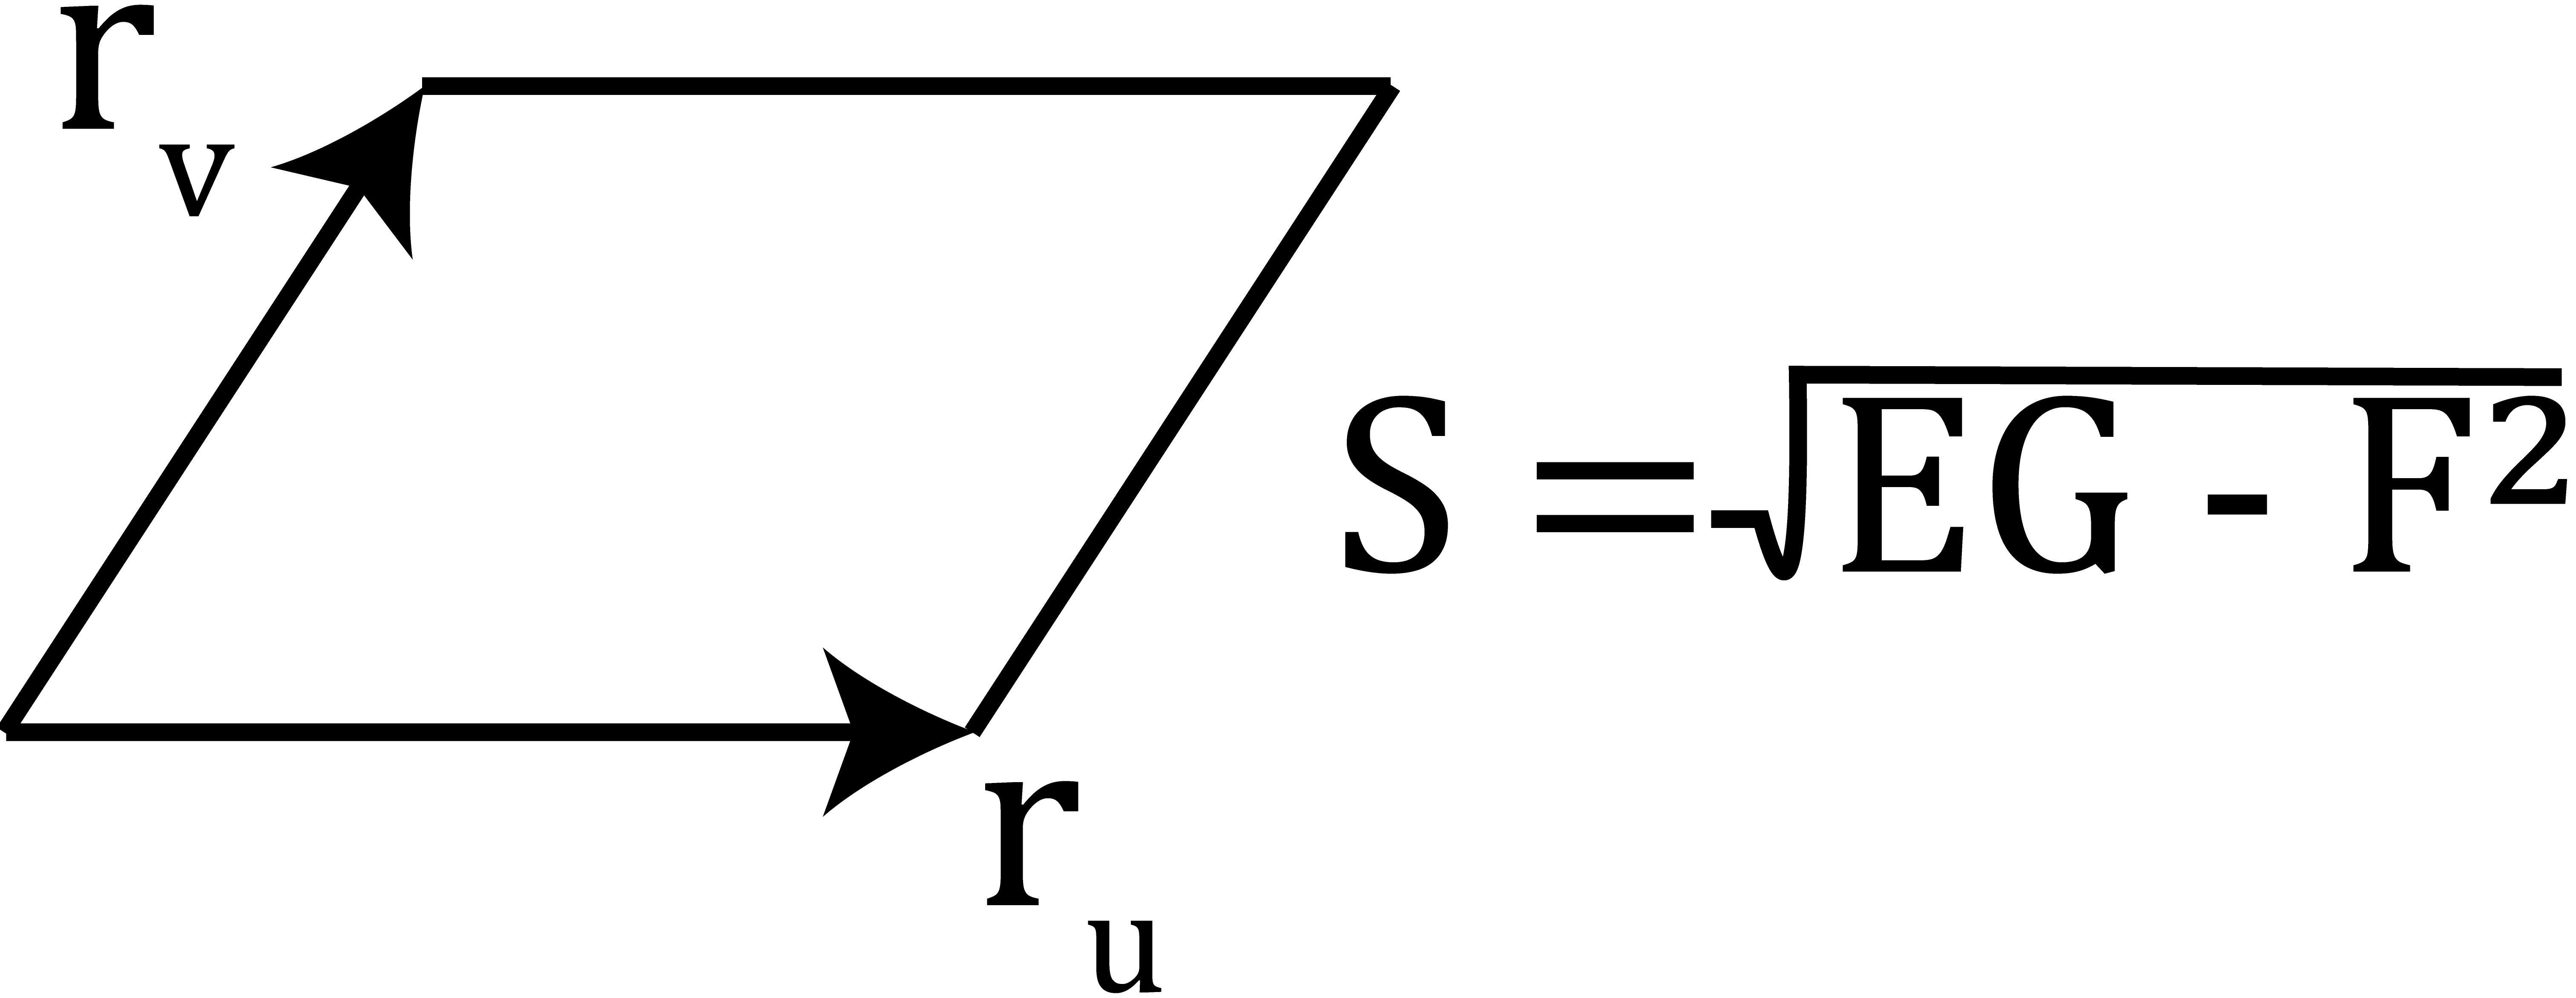
\includegraphics[width=6cm]{pics/9_1.png}
        \centering
    \end{figure}
    \[(2Nx + 2M)(Gx^2 + 2Fx + E) - (2Gx + 2F)(Nx^2 + 2Mx + L) = 0\]
    \begin{multline*}
        \cancel{NGx^3} + MGx^2 + 2NFx^2  + \cancel{2MFx} + FNx + ME-\\ - \cancel{GNx^3} - FNx^2 - 2GMx^2 - \cancel{2FMx} - GLx - FL = 0
    \end{multline*}
    \[x^2 (NF - MG) + x (EN - GL) + (ME - FL) = 0 \q |\cdot \xi^2\]
    \[\nu^2 \begin{vmatrix}
      F & G\\
      M & N
    \end{vmatrix} - \xi\nu \begin{vmatrix}
      G & E\\
      N & L
    \end{vmatrix} + \xi^2 \begin{vmatrix}
      E & F\\
      L & M
    \end{vmatrix} = 0\]
    \[\begin{vmatrix}
      \nu^2 & -\xi\nu & \xi^2\\
      E & F & G\\
      L & M & N
    \end{vmatrix} = 0\]

    \subsection{Вычисление главных кривизн, гауссовой кривизны и средней кривизны}
    Хотим понять, что происходит с различными k:
    \[\frac{\RNumb{2}(\xi, \nu)}{\RNumb{1}(\xi, \nu)} = k \qq (k \in \R)\]
    \[x = \frac{\nu}{\xi}\]
    \[\RNumb{2}(x) = k \RNumb{1}(x)\]
    \[Nx^2 + 2 Mx + L = k(Gx^2 + 2Fx +E)\]
    \[(N - kG)x^2 + 2(M - kF)x + (L - kE) = 0\]
    \begin{figure}[H]
        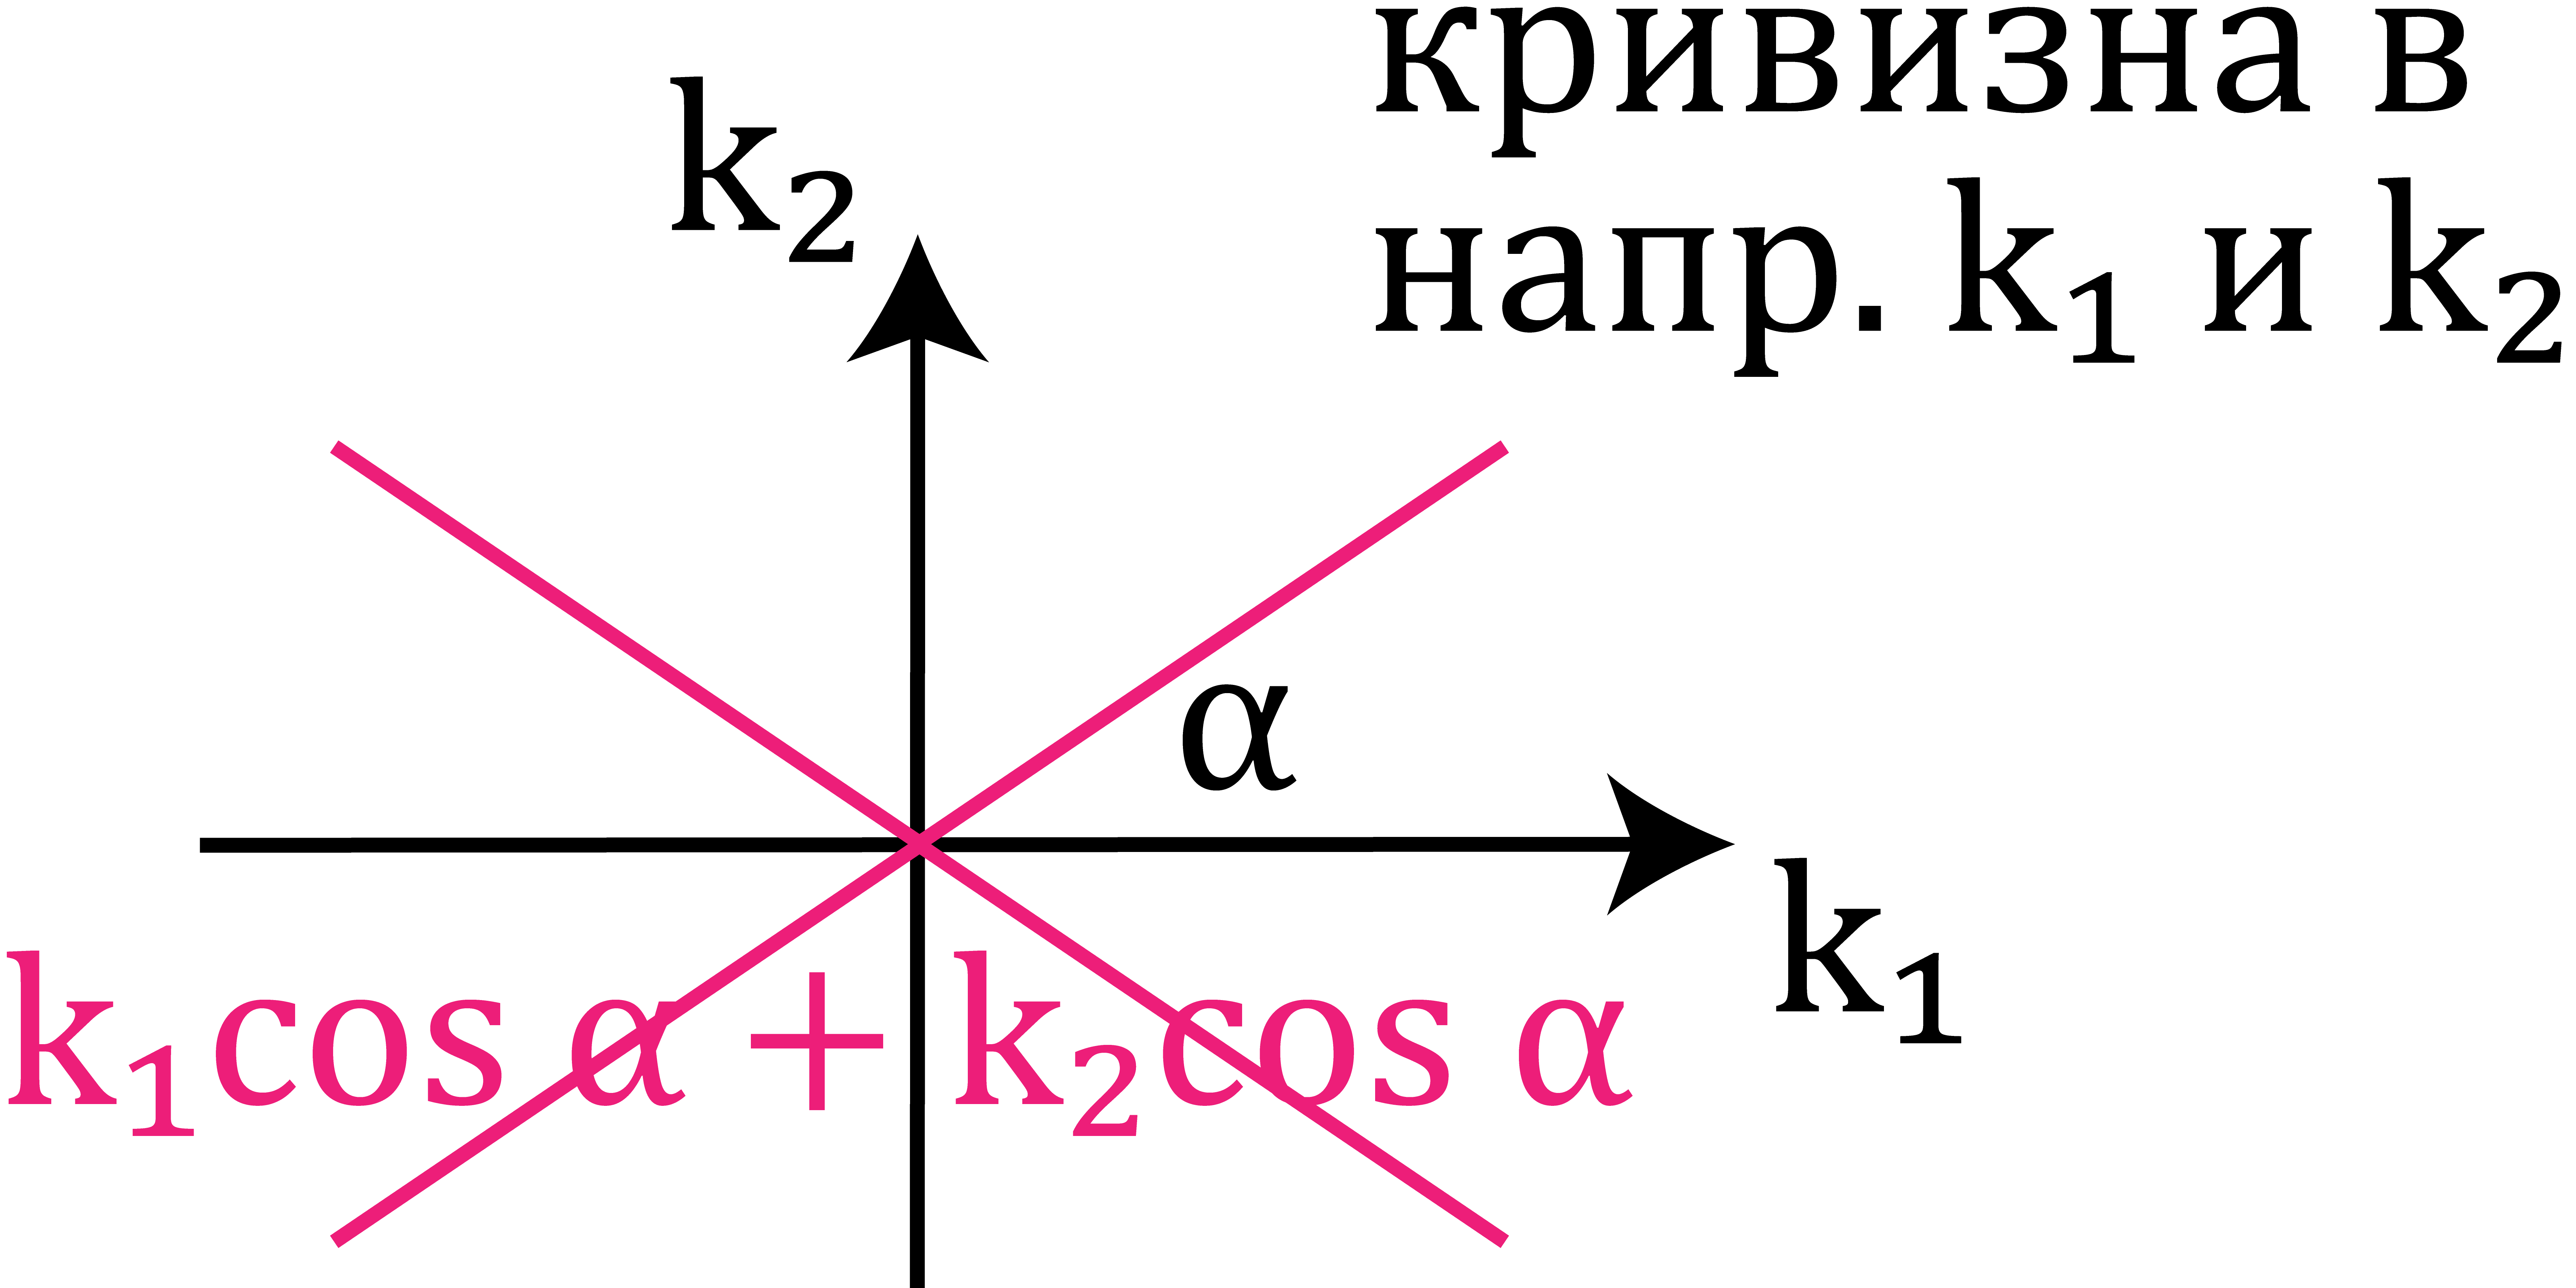
\includegraphics[width=6cm]{pics/9_2.png}
        \centering
    \end{figure}
    Если уравнение имеет 0 корней, такое число в качестве нормальной кривизны не достигается (если k слишком велико или слишком мало)

    Откуда могут взяться два корня? Пусть в одном направлении кривизна $k_1$, в другом $k_2$. Кривизна направления с углом $\alpha$ по ф-ле Эйлера $k_1 \cos^2 \alpha + k_2 \sin^2 \alpha$\\
    У симметричного относительно OX направления такая же кривизна. Вот откуда два корня

    А в каком случае корень $x_0$ единственный?
    \[\lra \text{напр. главное и $k = k_1$ или $k_2$}\]
    \[(M-kF)^2 = (N - kG)(L-kE)\]
    Его два решения --- главные кривизны\\
    <<решать мы его, конечно, не будем>>
    \[M^2 - k MF + k^2 F^2 = NL - k(GL + NE) + k^2 GE\]
    \[k^2 (GE - F^2) - k(GL + NE - 2MF) + (NL - M^2) = 0\]
    \[\Ra K = k_1 k_2 \os{\text{Виет}}{=} \frac{NL - M^2}{EG - F^2}\]
    \[H = \frac{k_1 + k_2}{2} = \frac{1}{2} \frac{GL - MF + NE}{EG - F^2}\]

    \subsection{Лемма о произведении смешанных произведений векторов.}
    \begin{lemma}
      $\ol{a}, \ol{b}, \ol{c}, \ol{d}, \ol{e}, \ol{f}$ --- вект из $\R^3$
      \[\Ra (\ol{a}, \ol{b}, \ol{c})(\ol{d}, \ol{e}, \ol{f}) = \begin{vmatrix}
          \ol{a}\cdot\ol{d} & \ol{a}\cdot\ol{e} & \ol{a}\cdot\ol{f}\\
          \ol{b}\cdot\ol{d} & \ol{b}\cdot\ol{e} & \ol{b}\cdot\ol{f}\\
          \ol{c}\cdot\ol{d} & \ol{c}\cdot\ol{e} & \ol{c}\cdot\ol{f}
      \end{vmatrix}\]
    \end{lemma}

    \begin{Proof}[д-во из учебника Александрова и Нецветаева]
        \[(\ol{a}, \ol{b}, \ol{c})(\ol{d}, \ol{e}, \ol{f}) = \begin{vmatrix}
            a_1 & a_2 & a_3\\
            b_1 & b_2 & b_3\\
            c_1 & c_2 & c_3
        \end{vmatrix} \cdot \begin{vmatrix}
            d_1 & d_2 & d_3\\
            e_1 & e_2 & e_3\\
            f_1 & f_2 & f_3
        \end{vmatrix} =\]
        \[= \begin{vmatrix}
            \begin{pmatrix}
                a_1 & a_2 & a_3\\
                b_1 & b_2 & b_3\\
                c_1 & c_2 & c_3
            \end{pmatrix}
            \cdot
            \begin{pmatrix}
                d_1 & e_1 & f_1\\
                d_2 & e_2 & f_2\\
                d_3 & e_3 & f_3
            \end{pmatrix}
        \end{vmatrix} = \begin{vmatrix}
            \ol{a}\cdot\ol{d} & \ol{a}\cdot\ol{e} & \ol{a}\cdot\ol{f}\\
            \ol{b}\cdot\ol{d} & \ol{b}\cdot\ol{e} & \ol{b}\cdot\ol{f}\\
            \ol{c}\cdot\ol{d} & \ol{c}\cdot\ol{e} & \ol{c}\cdot\ol{f}
        \end{vmatrix}\]
    \end{Proof}

    \begin{proof}[д-во от Солынина]
      Хотим $a \ra \ol{a} + \alpha \ol{b}$ (чтобы было ортогонально)
      \[\begin{vmatrix}
          (a + \alpha b)d & (a + \alpha b)e & (a + \alpha b)f\\
          bd & be & bf\\
          cd & ce & cf
      \end{vmatrix} \us{\text{с разл.}}{\os{\text{тот же трюк}}{=}} \begin{vmatrix}
          ad & ae & af\\
          bd & be & bf\\
          cd & ce & cf
      \end{vmatrix} + \ub{=0}{\begin{vmatrix}
          \alpha bd & \alpha be & \alpha bf\\
          bd & be & bf\\
          cd & ce & cf
      \end{vmatrix}}\]
      \[(a,b,c) \ra (a, b + \alpha a, c + \beta a + \gamma b)\]
      (трюк из первого семестра, $a \bot b \bot c \bot a$)\\
      Считаем, что они единичные:
      \[a = (1,0,0) \qq b = (0,1,0) \qq c = (0,0,1)\]
      \[d = (d_1, d_2, d_3) \qq e = (e_1, e_2, e_3) \qq f = (f_1, f_2, f_3)\]
      \[(d,e,f) = \begin{vmatrix}
        d_1 & e_1 & f_1\\
        d_2 & e_2 & f_2\\
        d_3 & e_3 & d_3
      \end{vmatrix}\]
    \end{proof}

    \subsection{Блистательная теорема Гаусса}
    \begin{Theorem}
      \[K = \frac{LN - M^2}{EG - F^2} \text{ выражается через $E,F,G$ и их произв.}\]
    \end{Theorem}

    \begin{Proof}
        \[\ol{n} = \frac{\ol{f}_u \times \ol{f}_v}{|f_u \times f_v|} = \frac{\ol{f}_u \times \ol{f}_v}{\sqrt{EG - F^2}}\]
        \[L = \ol{f}_{uu} \ol{n} = \frac{(f_{uu}, f_u, f_v)}{\sqrt{EG - F^2}}\]
        \[M = \ol{f}_{uv} \ol{n} = \frac{(f_{uv}, f_u, f_v)}{\sqrt{EG - F^2}}\]
        \[N = \ol{f}_{vv} \ol{n} = \frac{(f_{vv}, f_u, f_v)}{\sqrt{EG - F^2}}\]
        \begin{figure}[H]
            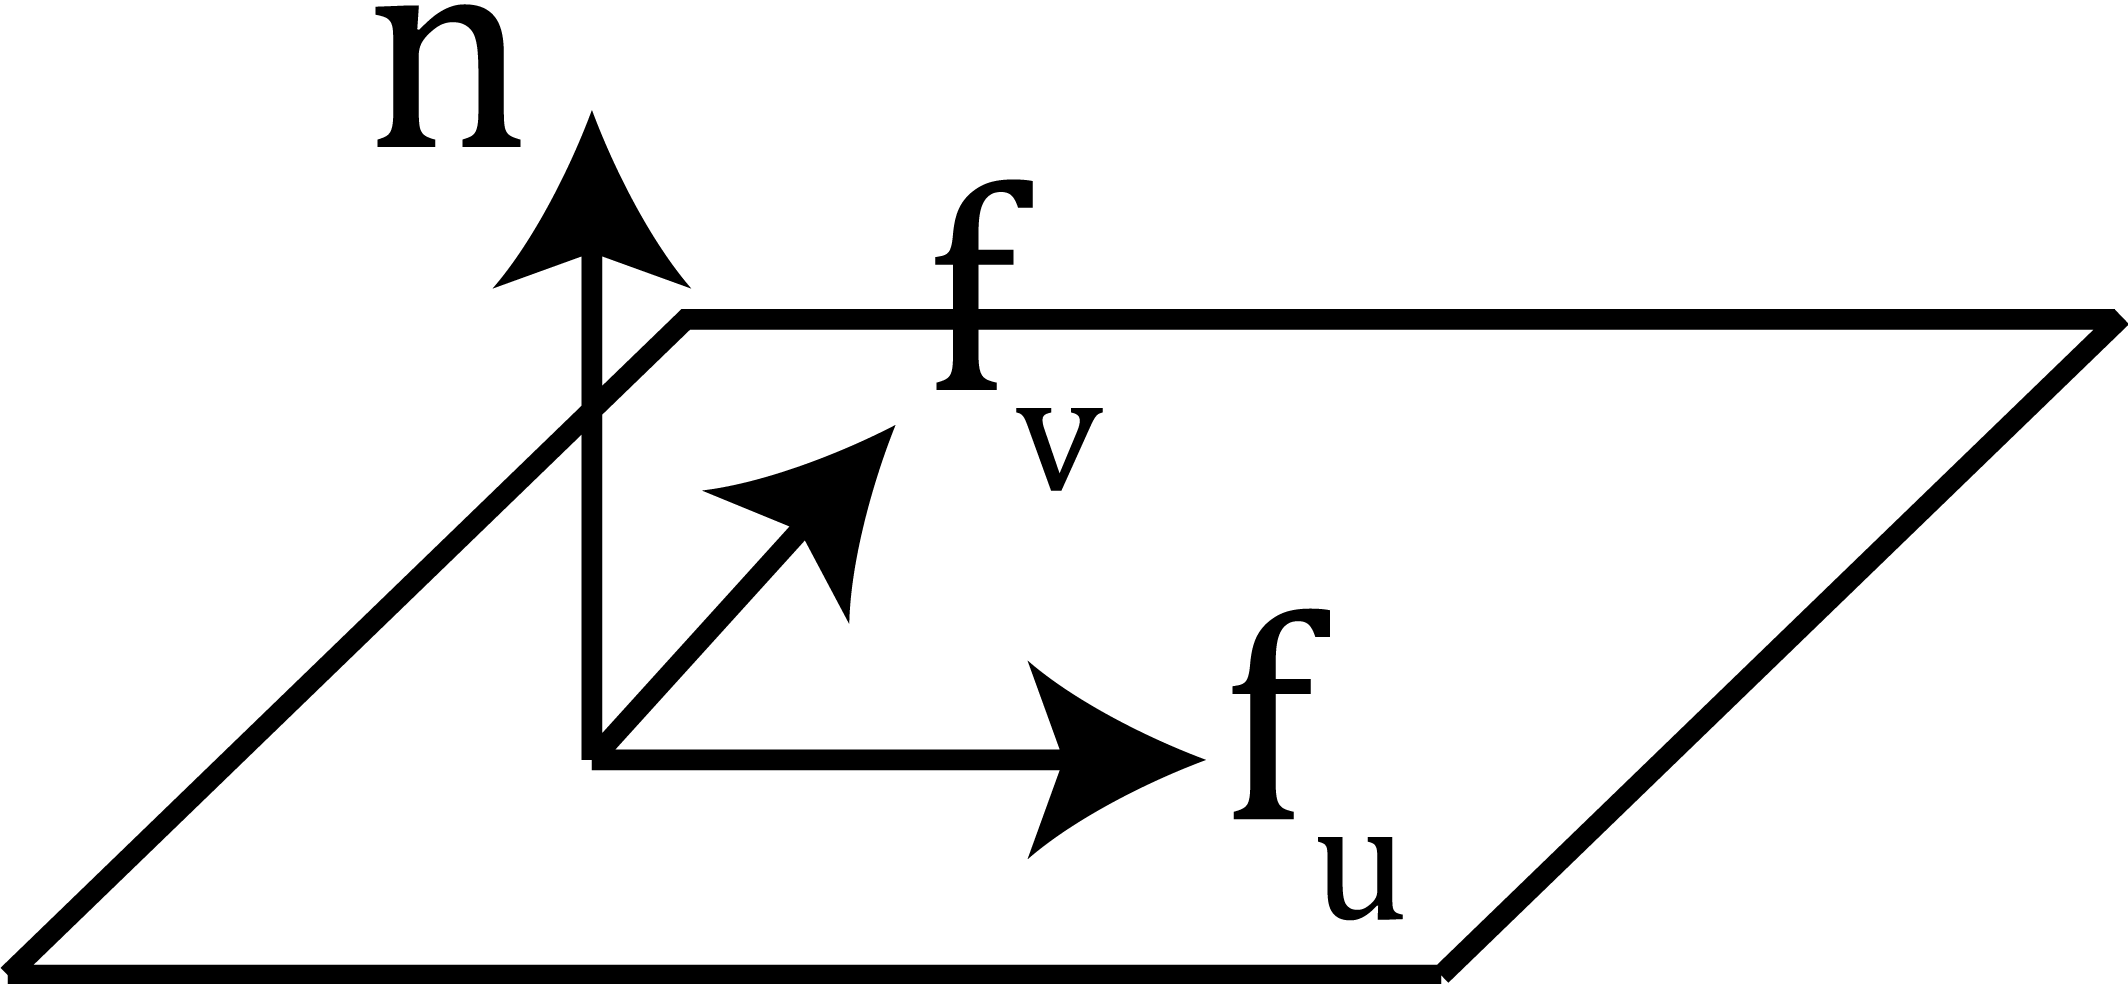
\includegraphics[width=4.5cm]{pics/9_3.png}
            \centering
        \end{figure}
        \[K = \frac{1}{(EG - F^2)^2} ( (f_{uu}, f_u, f_v)(f_{vv}, f_u, f_v) - (f_{uv}, f_u, f_v)(f_{uv}, f_u, f_v) )\]
        \[= \frac{1}{(EG - F^2)^2} \begin{vmatrix}
            f_{uu}f_{vv} & f_{uu}f_{u} & f_{uu}f_{v}\\
            f_{u}f_{vv} & f_{u}f_{u} & f_{u}f_{v}\\
            f_{v}f_{vv} & f_{v}f_{u} & f_{v}f_{v}
        \end{vmatrix} - \begin{vmatrix}
            f_{uv}f_{uv} & f_{uv}f_{u} & f_{uv}f_{v}\\
            f_{u}f_{uv} & f_{u}f_{u} & f_{u}f_{v}\\
            f_{v}f_{uv} & f_{v}f_{u} & f_{u}f_{v}
        \end{vmatrix} =\]
        \[E_u = (f_u f_u)_u = 2 f_u f_{uu}\]
        \[E_v = (f_u^2)_v = 2 f_u f_{uv}\]
        \[F_u = (f_u f_v)_u = f_{uu}f_v + f_u f_{uv}\]
        \[F_v = (f_u f_v)_v = f_u f_{vv} + f_v f_{uv}\]
        \[G_u = (f_v f_v)_u = 2 f_v f_{uv}\]
        \[G_v = (f_v f_v)_v = 2 f_{vv} f_v\]
        \[f_u f_{uv} = \frac{1}{2} E_v\]
        \[f_{uu} f_v = F_u - \frac{1}{2} E_v\]
        \[f_{vv} f_u = F_v - \frac{1}{2} G_u\]
        \[ = \frac{1}{(EG - F^2)^2} \Br{\begin{vmatrix}
            f_{uu} f_{vv} & \frac{1}{2} E_u & F_u - \frac{1}{2} E_v\\
            F_v - \frac{1}{2} G_u & E & F\\
            \frac{1}{2} G_v & F & G
        \end{vmatrix} - \begin{vmatrix}
            f_{uv}^2 & \frac{1}{2}E_v & \frac{1}{2} G_u\\
            \frac{1}{2}E_v & E & F\\
            \frac{1}{2}F_u & F & G
            \end{vmatrix}} =
        \]
        \[ = \frac{1}{(EG - F^2)^2} \Br{\begin{vmatrix}
            f_{uu} f_{vv} - f_{uv}^2 & \frac{1}{2} E_u & F_u - \frac{1}{2} E_v\\
            F_v - \frac{1}{2} G_u & E & F\\
            \frac{1}{2} G_u & F & G
            \end{vmatrix} - \begin{vmatrix}
            0 & \frac{1}{2}E_v & \frac{1}{2} G_u\\
            \frac{1}{2}E_v & E & F\\
            \frac{1}{2}G_u & F & G
            \end{vmatrix}}
        \]
        \[F_{uv} = (f_{uu} f_v)_v + (f_u f_{uv})_v = f_{uuv} f_v + \ul{f_{uu}f_{vv}} + \ul{f_{uv}f_{uv}} + f_u f_{uvv}\]
        \[G_{uu} = 2 f_{uv}^2 + 2 f_v f_{uvu}\]
        \[E_{vv} = 2 f_{uv}^2 + 2 f_u f_{uvv}\]
        \[\Ra f_{uu} f_{vv} - f^2_{uv} = F_{uv} - \frac{1}{2}(G_{uu}+E_{vv})\]
        Можем заменить теперь в определителе и теорема будет доказана
    \end{Proof}
\end{document}
